%%%%%%%%%%%%%%%%%%%%%%%%%%%%%%%%%%%%%%%%%%%%%%%%%%%%%%%%%%%%%%%

% Set up document

\documentclass{beamer}
\usecolortheme{owl}
\setbeamersize{text margin left=5mm,text margin right=5mm}

% Used to create a section slide between section
\AtBeginSection[]{
  \begin{frame}
  \vfill
  \centering
  \begin{beamercolorbox}[sep=8pt,center,shadow=true,rounded=true]{title}
    \usebeamerfont{title}\insertsectionhead\par%
  \end{beamercolorbox}
  \vfill
  \end{frame}
}

% Remove default navigation symbols and add just  page number
\setbeamertemplate{navigation symbols}{} % Clear default navigation
\addtobeamertemplate{navigation symbols}{}{%
    \usebeamerfont{footline}%
    \usebeamercolor[fg]{footline}%
    \hspace{1em}%
    \insertframenumber/\inserttotalframenumber
}


%%%%%%%%%%%%%%%%%%%%%%%%%%%%%%%%%%%%%%%%%%%%%%%%%%%%%%%%%%%%%%%

% Title page

\title{Stroke Audit Machine Learning (SAMueL) \\ Patient and Carers Involvement Group}

%\institute{Overleaf}
\date{October 2022}


\begin{document}

\frame{\titlepage}

%%%%%%%%%%%%%%%%%%%%%%%%%%%%%%%%%%%%%%%%%%%%%%%%%%%%%%%%%%%%%%%

%%%%%%%%%%%%%%%%%%%%%%%%%%%%%%%%%%%%%%%%%%%%%%%%%%%%%%%%%%%%%%%

\begin{frame}
\frametitle{Two types of stroke}
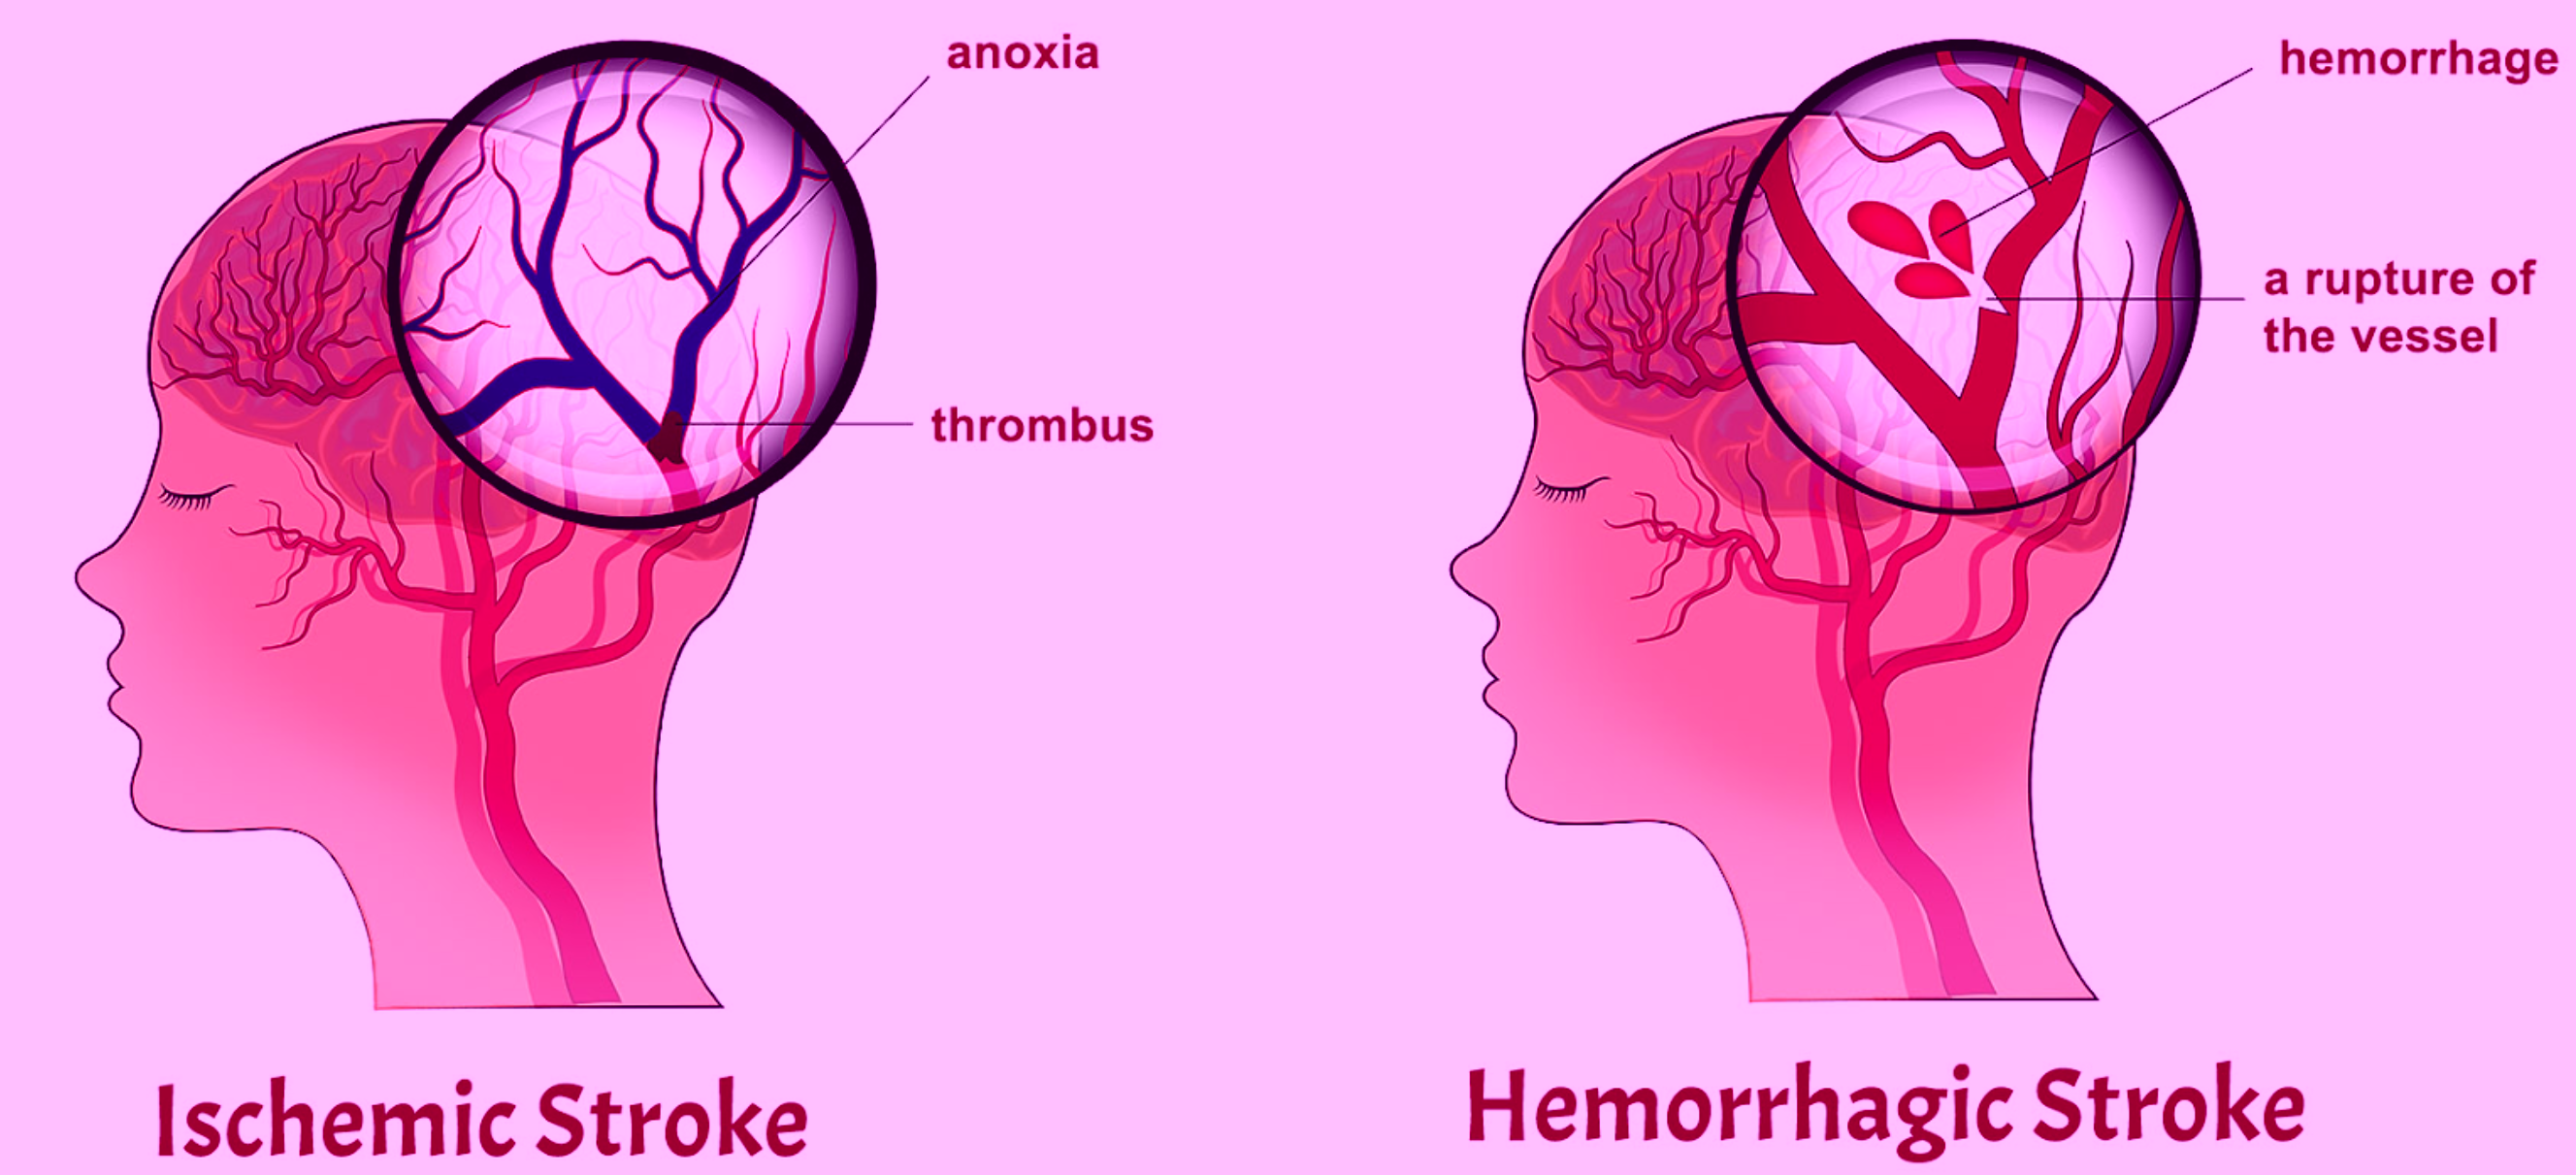
\includegraphics[width=1.0\textwidth]{./images/stroke_types}
\end{frame}

%%%%%%%%%%%%%%%%%%%%%%%%%%%%%%%%%%%%%%%%%%%%%%%%%%%%%%%%%%%%%%%

\begin{frame}
\frametitle{Thrombolysis}
Thrombolysis aims to break down a clot by activating the body's own clot breakdown mechanisms.

\vspace{5mm}

Thrombolysis is given as an injection followed by an infusion (\emph{drip}).

\begin{center}
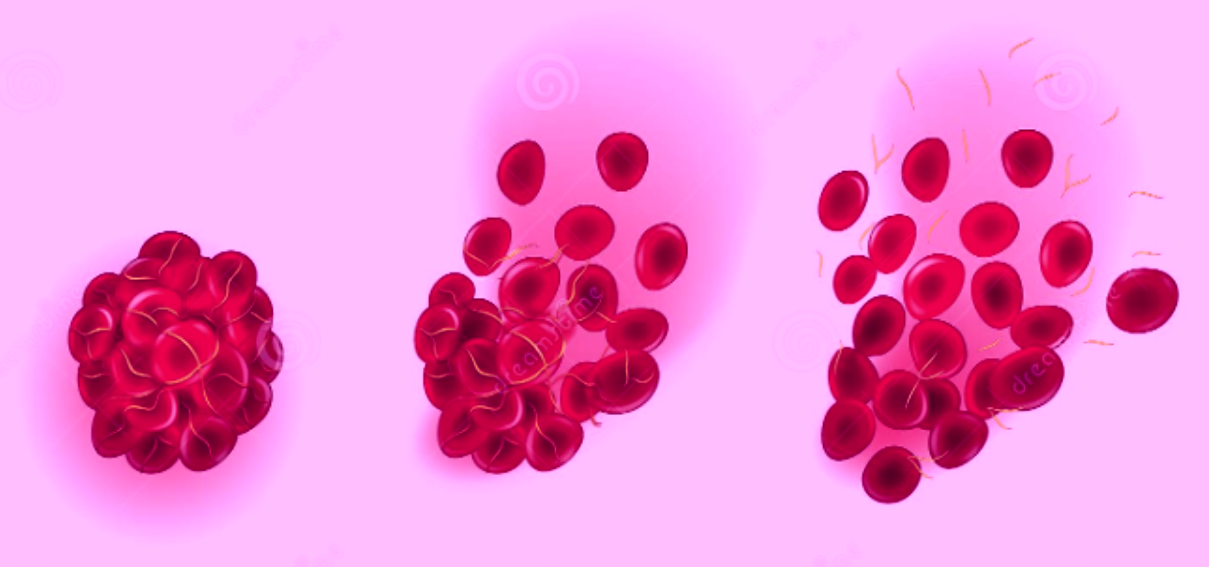
\includegraphics[width=0.8\textwidth]{./images/thrombolysis_mechanism}
\end{center}
\end{frame}

%%%%%%%%%%%%%%%%%%%%%%%%%%%%%%%%%%%%%%%%%%%%%%%%%%%%%%%%%%%%%%%

\begin{frame}
\frametitle{What is the problem?}
\begin{itemize}
    \setlength\itemsep{5mm}
    \item Expert clinical opinion is that one in five people (20\%) should be receiving thrombolysis.
    \item In England, about 1 in 9 people (11\%) actually receive thrombolysis.
    \item Nearly half the people who \emph{could} benefit from thrombolysis do not currently have the opportunity.
    \item Use of thrombolysis in England has been stable for 10 years.
\end{itemize}
\end{frame}


%%%%%%%%%%%%%%%%%%%%%%%%%%%%%%%%%%%%%%%%%%%%%%%%%%%%%%%%%%%%%%%

\begin{frame}
\frametitle{Breaking down the emergency stroke pathway into key steps}
\begin{center}
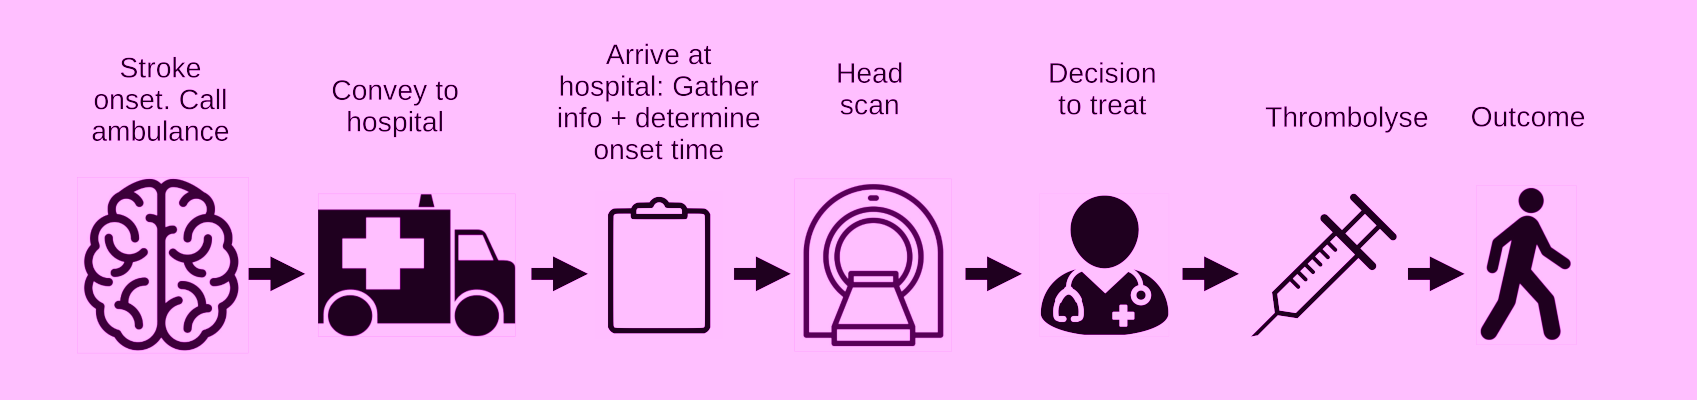
\includegraphics[width=1.05\textwidth]{./images/pathway}
\end{center}
We can model key changes to pathway:
\begin{itemize}
    \item What if the pathway were faster?
    \item What if hospital determined the stroke onset time in more patients?
    \item What if clinical decision-making was like that of \emph{benchmark} hospitals? (Predict what treatment a patient would receive at other hospitals).
\end{itemize}
\end{frame}

%%%%%%%%%%%%%%%%%%%%%%%%%%%%%%%%%%%%%%%%%%%%%%%%%%%%%%%%%%%%%%%

\begin{frame}
\frametitle{Machine learning overview}
\begin{center}
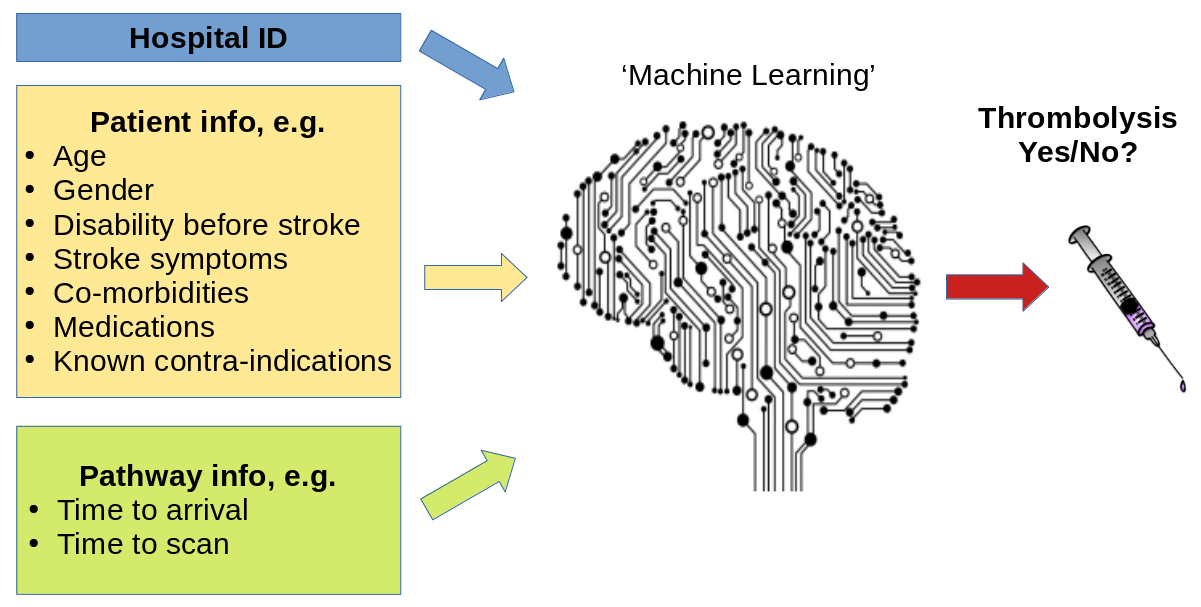
\includegraphics[width=0.90\textwidth]{./images/ml_model_high_level}
\end{center}

Machine learning (and nearly all \emph{artificial intelligence}) is based on the simple principle of recognising similarity to what has been seen before.
\vspace{3mm}

We accessed 240,000 emergency stroke admissions in England and Wales over three years. That is a lot of examples to learn from!
\end{frame}




%%%%%%%%%%%%%%%%%%%%%%%%%%%%%%%%%%%%%%%%%%%%%%%%%%%%%%%%%%%%%%%

\begin{frame}
\frametitle{SAMueL-1 Summary: What is the problem?}
\begin{center}
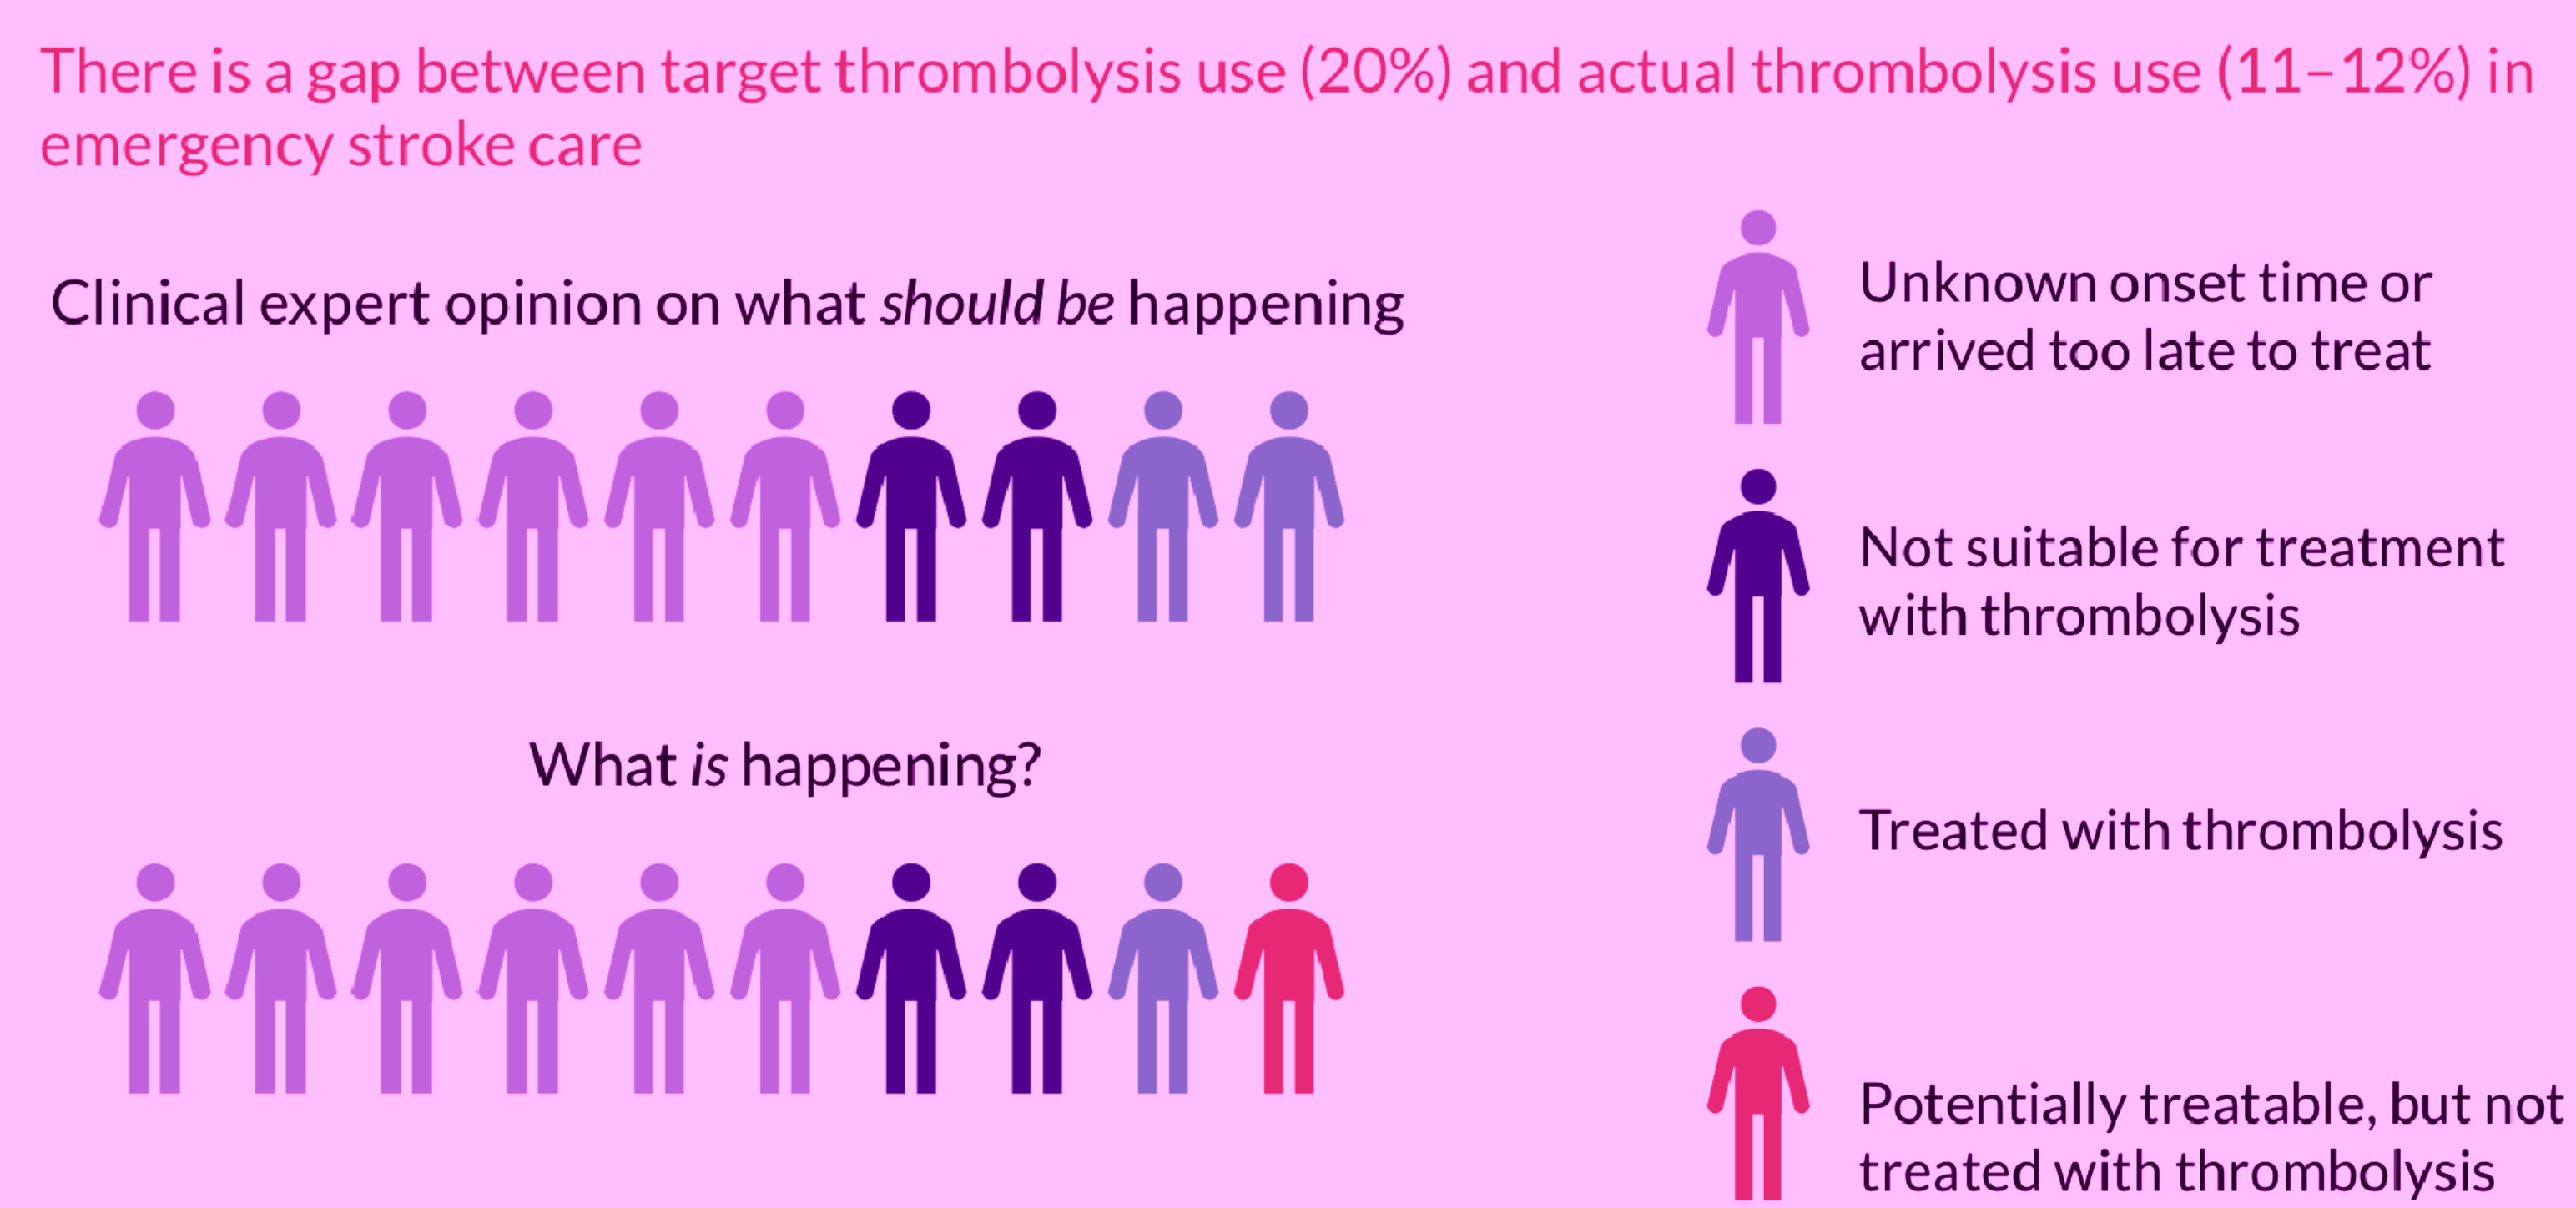
\includegraphics[width=1.0\textwidth]{./images/sam_summary_pt_1}
\end{center}
\end{frame}

\begin{frame}
\frametitle{SAMueL-1 Summary: What did we test?}
\begin{center}
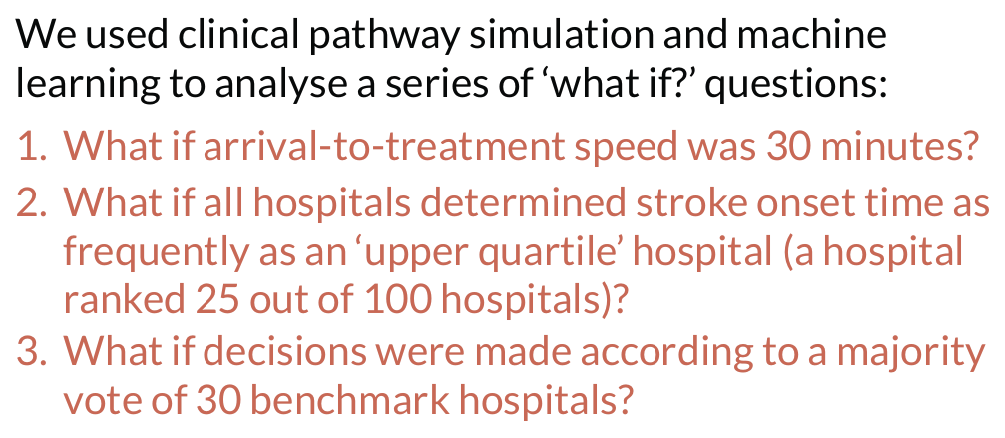
\includegraphics[width=1.0\textwidth]{./images/sam_summary_pt_2}
\end{center}

For each hospital we use their own patients to ask these questions, to allow for differences in local patient populations.
\end{frame}

\begin{frame}
\frametitle{SAMueL-1 Summary: What did we find?}
\begin{center}
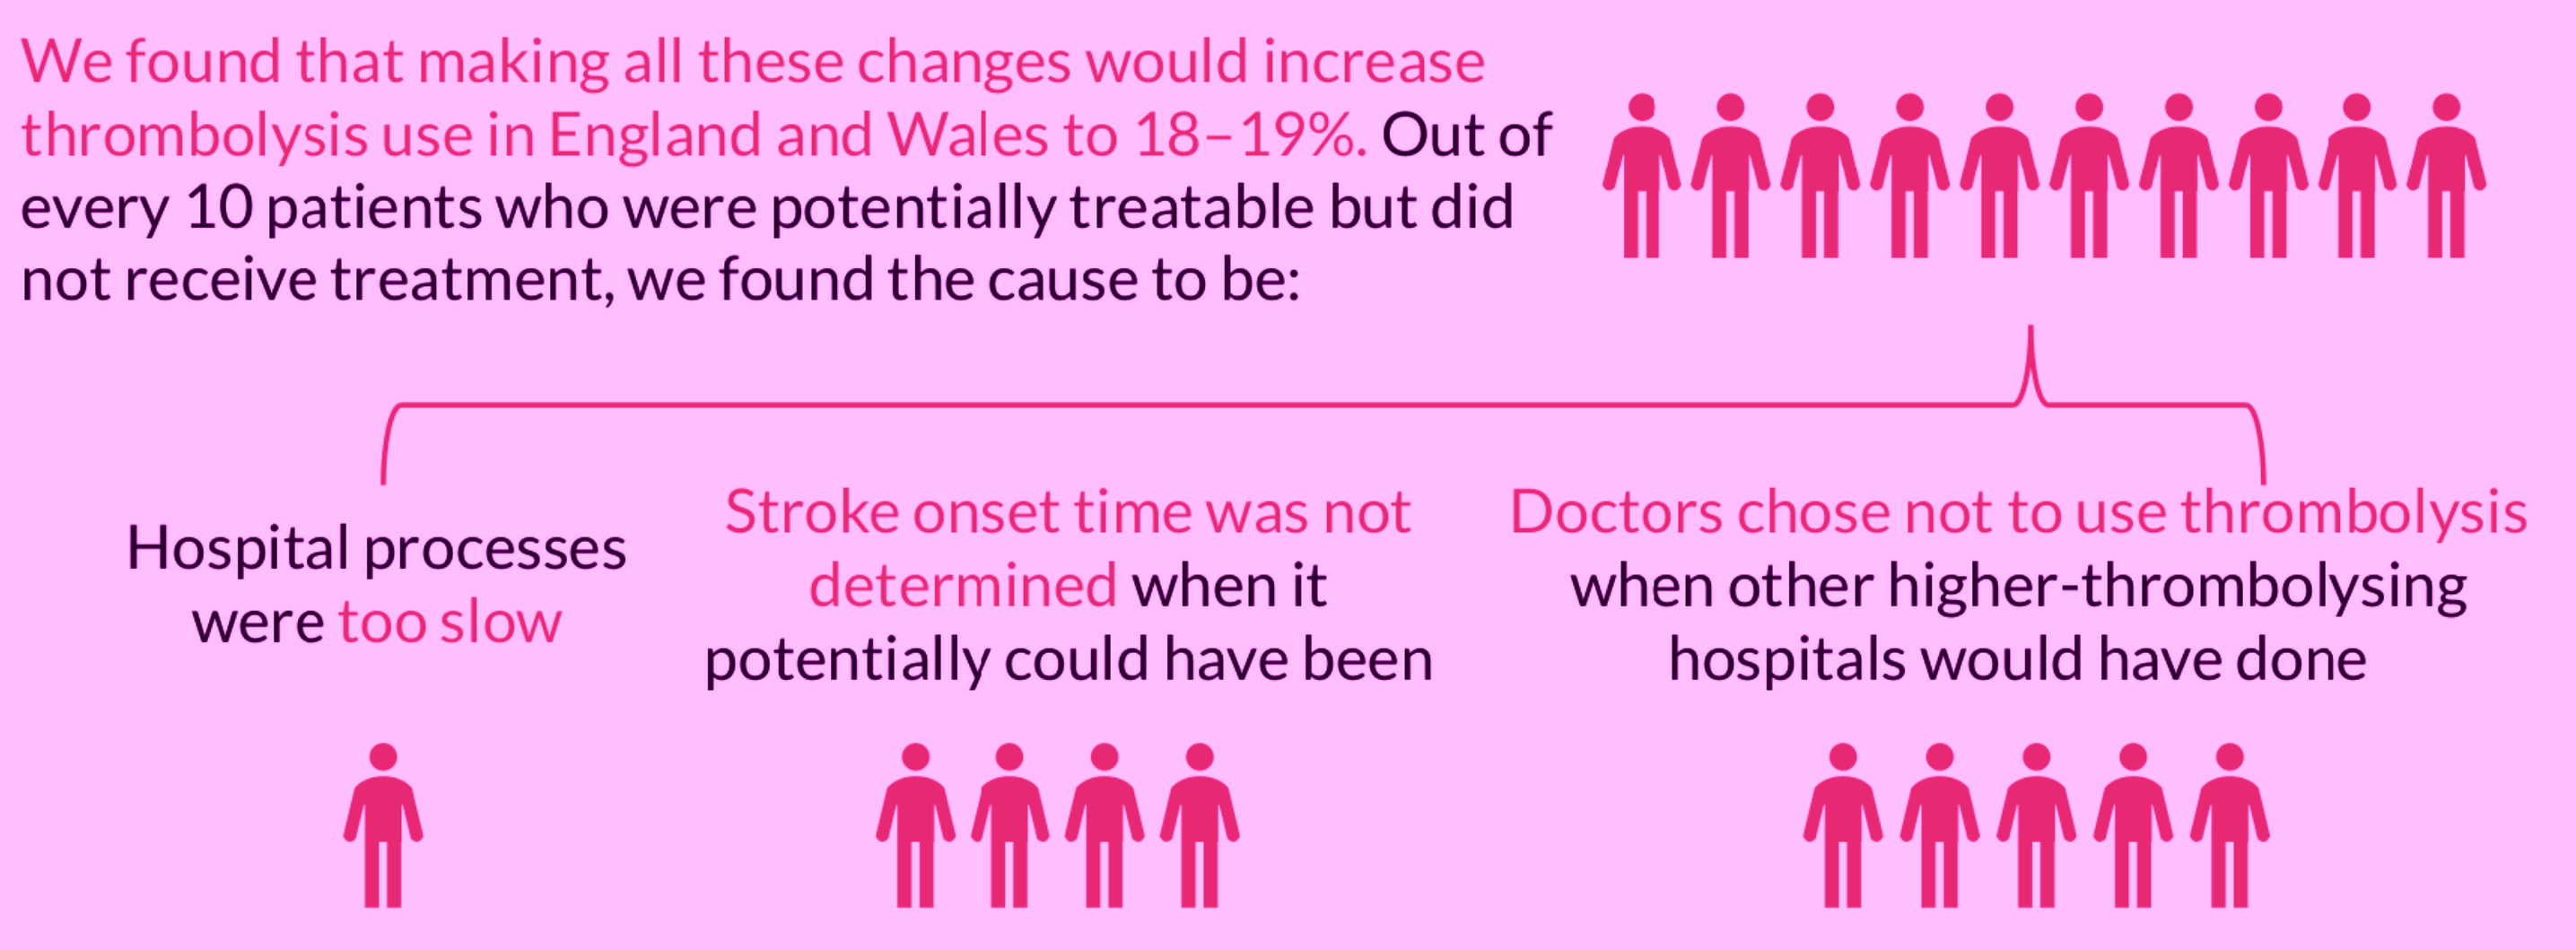
\includegraphics[width=1.0\textwidth]{./images/sam_summary_pt_3}
\end{center}
\end{frame}

%%%%%%%%%%%%%%%%%%%%%%%%%%%%%%%%%%%%%%%%%%%%%%%%%%%%%%%%%%%%%%%

\begin{frame}
\frametitle{Applying our models at hospital level}

\begin{center}
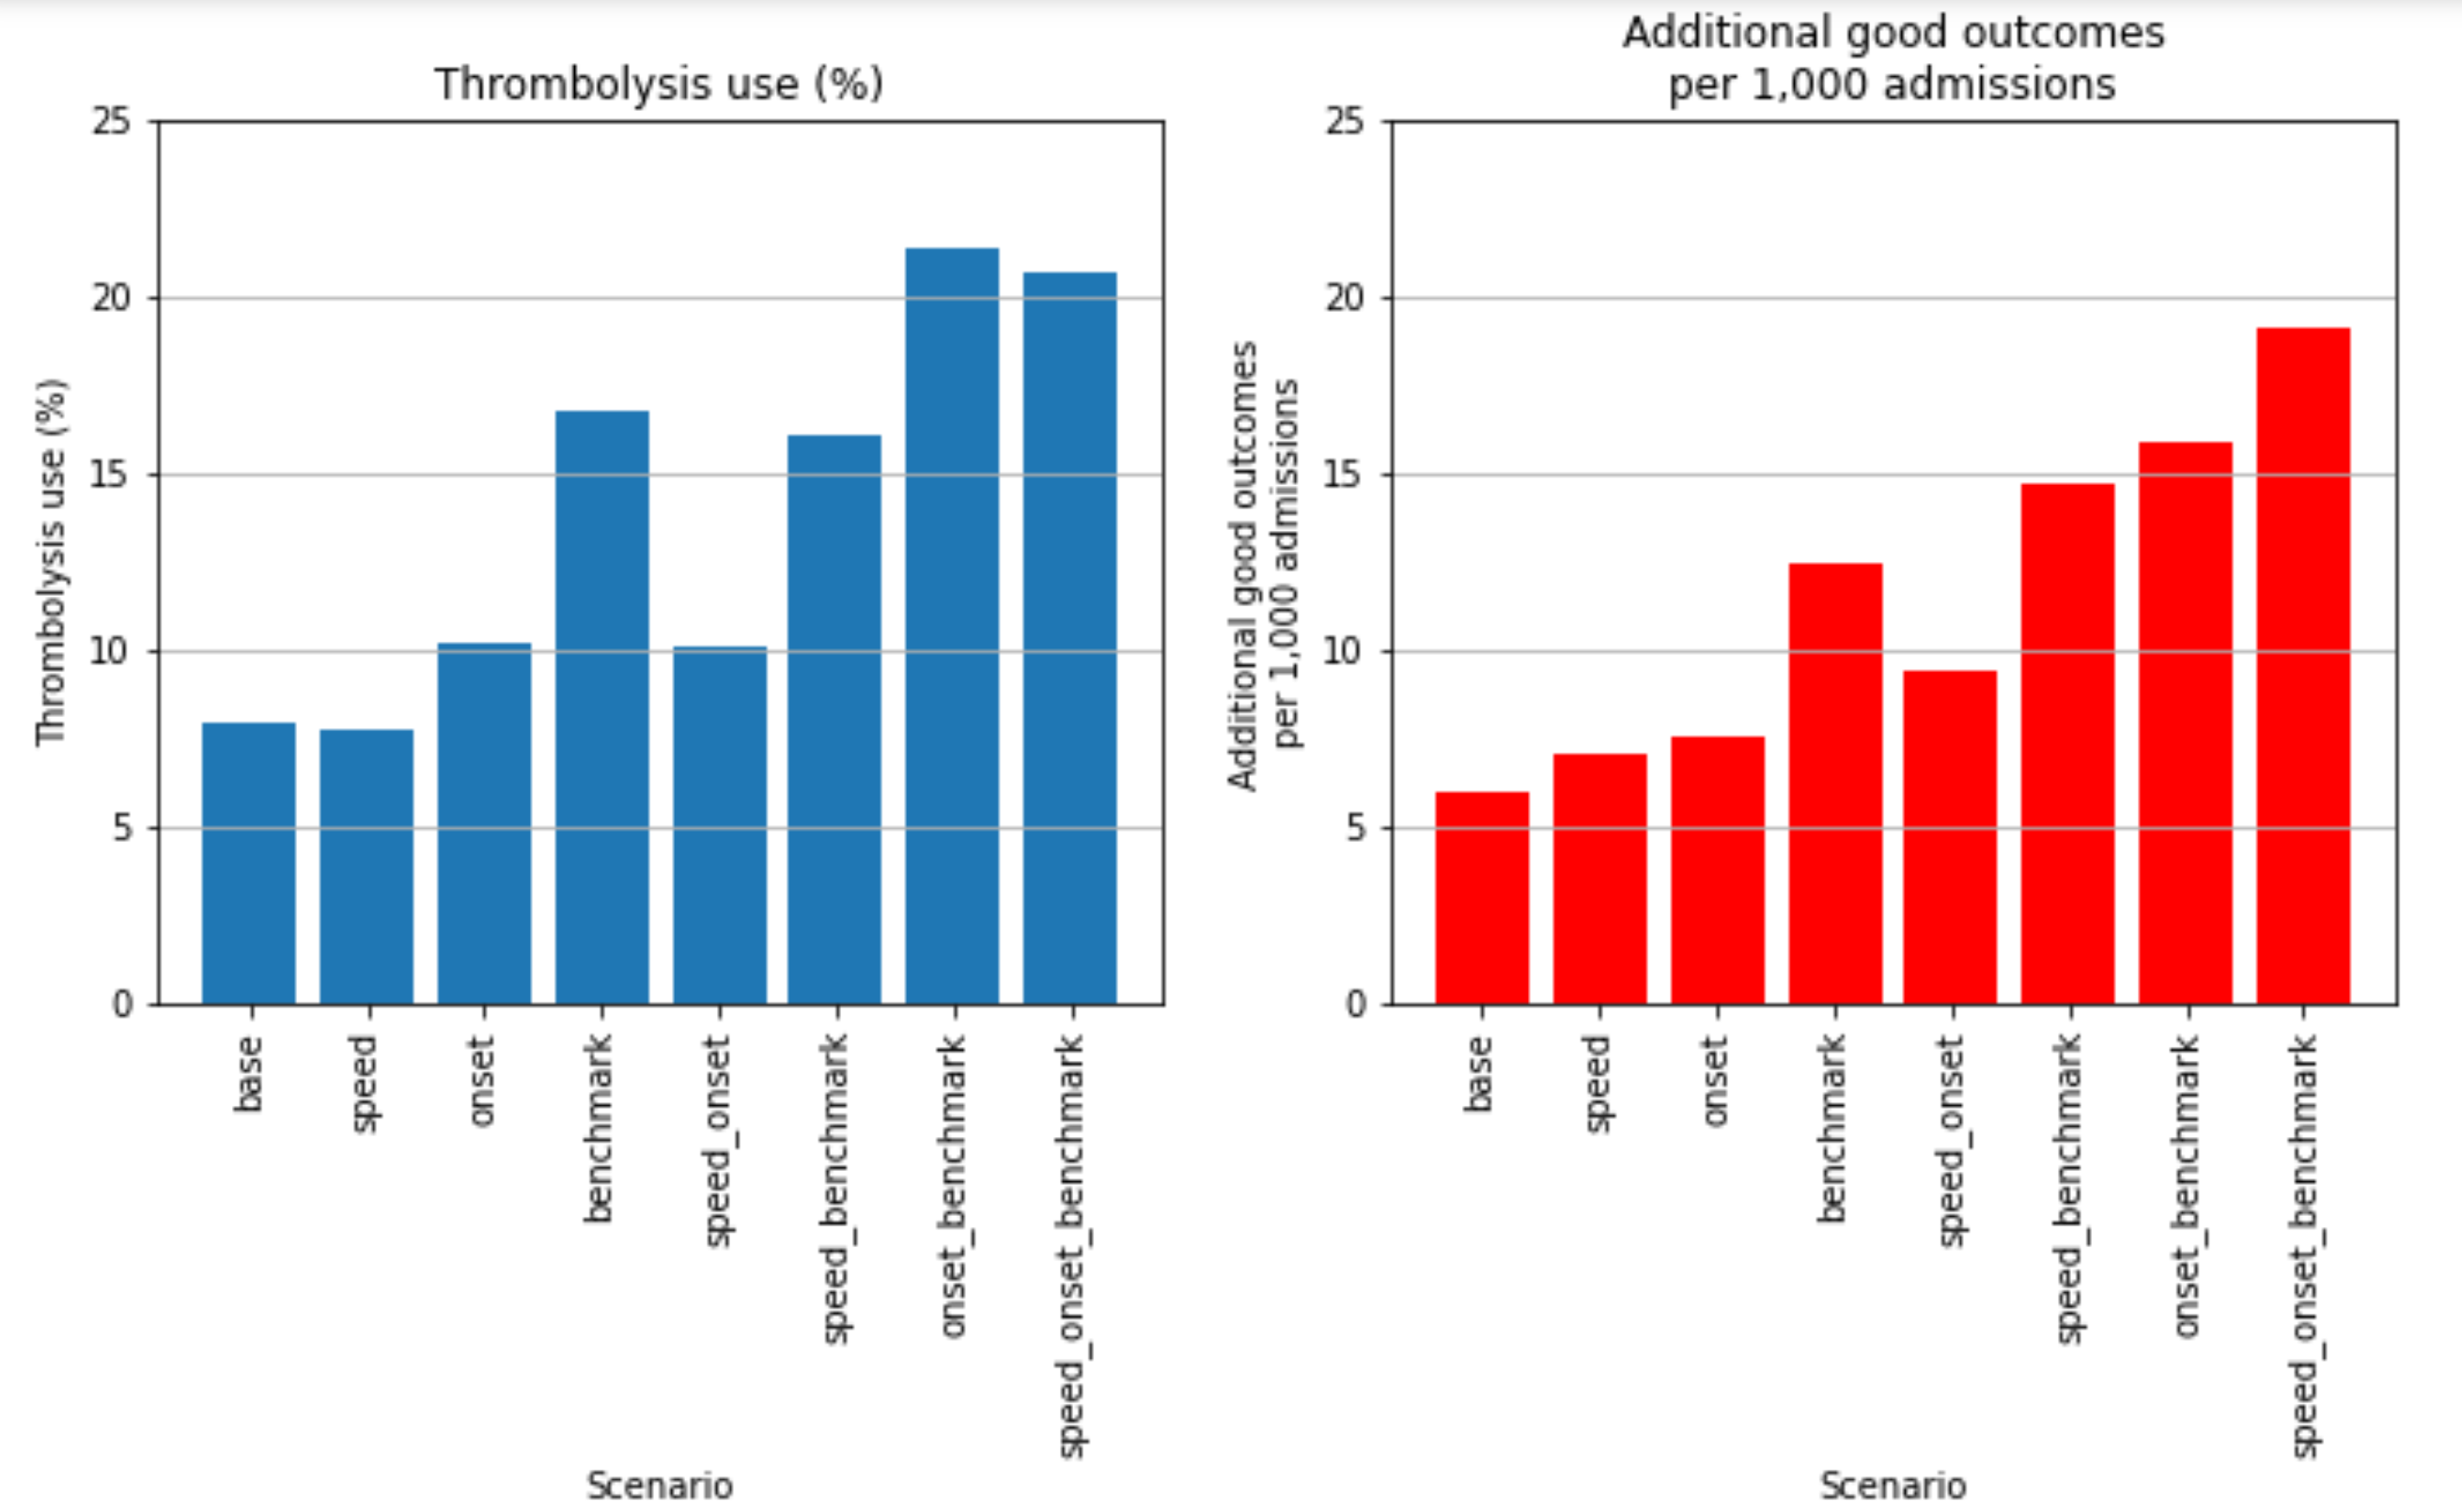
\includegraphics[width=0.95\textwidth]{./images/hosp_scenario_1}
\end{center}

\end{frame}

%%%%%%%%%%%%%%%%%%%%%%%%%%%%%%%%%%%%%%%%%%%%%%%%%%%%%%%%%%%%%%%

\begin{frame}
\frametitle{What questions are we asking in SAMueL-2?}
\begin{itemize}
    \setlength\itemsep{5mm}
    \item What patients do clinicians agree and disagree on, when considering when they should receive thrombolysis?
        \begin{itemize}
        \item We'll discuss that at our next meeting!
    \end{itemize}
    \item How do \emph{organisational factors} (such as use of specialist stroke nurses) affect the thrombolysis pathway and decision-making?

    \item How best can we engage clinicians in our work, and prompt them to reconsider their emergency stroke pathway and/or decision-making?
    
    \begin{itemize}
        \item Communication of general findings.
        \item Web application for individual hospitals.
        \item A 'hospital profile` for each hospital.
    \end{itemize}
\end{itemize}

\end{frame}

%%%%%%%%%%%%%%%%%%%%%%%%%%%%%%%%%%%%%%%%%%%%%%%%%%%%%%%%%%%%%%%

\end{document}








